% !TEX root = ../main.tex
\section{Деякі закони розподілу випадкових величин}

\subsection{Біноміальний розподіл}
\noindent\textbf{Означення:}
    ДВВ $\xi$ розподілена за \emph{біноміальним законом}, 
    якщо набуває значень $0,1,...,n$ з ймовірностями \begin{equation}
        \P\left\{\xi = k\right\} = C_n^k p^k q^{n-k}, q = 1 - p
    \end{equation}
\textbf{Коротке позначення:} $\xi \sim \mathrm{Bin}(n, p)$.
    $n$ і $p$ --- параметри закону, $n\in \mathbb{N}$, $p\in (0;1)$.

Окремим важливим випадком біноміального закону є \emph{розподіл Бернуллі}: $\xi \sim \mathrm{Bin}(1, p)$.
За законом Бернуллі розподілені випадкові величини-індикатори $I_A = \begin{cases}
    0, & \text{подія A не відбулась}\\ 1, & \text{подія А відбулась}
\end{cases}$ при $\P(A) = p$.

\noindent\textbf{Ряд розподілу:}

\begin{tabular}{|c|c|c|c|c|c|}
    \hline
    $\xi$ & $0$ & $1$ & $2$ & $..$. & $n$ \\
    \hline
    $p$ & $q^n$ & $npq^{n-1}$ & $C_n^2 p^2 q^{n-2}$ & $...$ & $p^n$ \\
    \hline
\end{tabular}

\noindent\textbf{Функція розподілу:}

\begin{tabular}{c c}
    $
        F_\xi(x) = \begin{cases}
            0, & x \leq 0 \\
            q^n, & 0 < x \leq 1 \\
            q^n + npq^{n-1}, & 1 < x \leq 2 \\
            \dots \\
            1, & x > n
        \end{cases}
    $ &
    \begin{tikzpicture}[baseline={(current bounding box.center)}, yscale=2.5]
        \pgfmathsetmacro{\p}{0.6};
        \pgfmathsetmacro{\q}{1-\p};
        \pgfmathsetmacro{\n}{5};
        \draw [->] (-1,0) -- (\n+1, 0);
        \draw [->] (0, -0.1) -- (0, 1.2);
        \draw [ultra thick] (-1, 0) -- (0,0);
        \draw [ultra thick] [<-] (0,\q^\n) -- (1, \q^\n);
        \draw [ultra thick] [<-] (1, {\q^\n + \n*\p*\q^(\n-1)}) -- (2, {\q^\n + \n*\p*\q^(\n-1)});
        \draw [ultra thick] [<-] (2, {\q^\n + \n*\p*\q^(\n-1) + (\n*(\n-1)/2)*\p^2*\q^(\n-2)}) -- (3, {\q^\n + \n*\p*\q^(\n-1) + (\n*(\n-1)/2)*\p^2*\q^(\n-2)});
        \draw [ultra thick] [<-] (3, {1 - (\q^\n + \n*\p*\q^(\n-1) + (\n*(\n-1)/2)*\p^2*\q^(\n-2))}) -- (4, {1 - (\q^\n + \n*\p*\q^(\n-1) + (\n*(\n-1)/2)*\p^2*\q^(\n-2))});
        \draw [ultra thick] [<-] (4, {1 - (\q^\n + \n*\p*\q^(\n-1))}) -- (5, {1 - (\q^\n + \n*\p*\q^(\n-1))});
        \draw [ultra thick] [<-] (5, 1) -- (6, 1);
        \node [below left] at (0, 0) {0};
        \foreach \k in {1,...,\n}:
            \node [below] at (\k, 0) {\k};
        \draw [dashed] (0, 1) -- (\n, 1);
        \node [left] at (0, 1) {1};
        \node [right] [align=center] at (3.5, 0.2) {Приклад для \\ $n = \n, p = \p$};
        \node [below] at (\n+1, 0) {$x$};
        \node [left] at (0, 1.2) {$F_\xi(x)$};
    \end{tikzpicture}
\end{tabular}

Для дослідження числових характеристик скористаємося генератрисою розподілу:

$G_\xi(z) = \sum\limits_{k=0}^{n} \P\left\{\xi = k\right\} z^k = \sum\limits_{k=0}^{n} C_n^k p^k q^{n-k} z^k = (pz+q)^n$.
$G'_\xi(z) = np(pz+q)^{n-1}$, $G''_\xi(z) = n(n-1)p^2(pz+q)^{n-2}$.

$G'_\xi(1) = np(p+q)^{n-1} = np$, $G''_\xi(1) = n(n-1)p^2 = n^2p^2 - np^2$, $G''_\xi(1) + G'_\xi(1) - \left( G'_\xi(1)\right)^2 = n^2p^2 - np^2 + np - n^2p^2 = np(1-p) = npq$.
Отже, знайдено значення математичного сподівання та дисперсії.

\noindent\textbf{Числові характеристики:}
\begin{enumerate}
    \item $\E\xi = np$.
    \item $\D\xi = npq$, $\sigma_\xi = \sqrt{npq}$.
    \item ${Mo}\xi = \begin{cases}
        \left[np+p\right], & \text{якщо } np+p \text{ не ціле}\\
        np+p, np-q, & \text{якщо } np+p \text{ ціле}
    \end{cases}$ --- як найбільш ймовірна кількість успіхів у схемі Бернуллі.
    \item ${Me}\xi$ --- одне зі значень $\left[np\right] - 1$, $\left[np\right]$, $\left[np\right] + 1$.
\end{enumerate}

\noindent\textbf{Застосування:} якщо проводиться $n$ незалежних випробувань з ймовірністю успіху $p$, 
то $\xi \sim \mathrm{Bin}(n, p)$ задає кількість успіхів.

\subsection{Геометричний розподіл}
\noindent\textbf{Означення:}
    ДВВ $\xi$ розподілена за \emph{геометричним законом}, 
    якщо набуває значень $1,2,3,..$ з ймовірностями \begin{equation}
        \P\left\{\xi = k\right\} = pq^{k-1}, q = 1 - p
    \end{equation}
    \textbf{Коротке позначення:} $\xi \sim \mathrm{Geom}(p)$.
    $p$ --- параметр закону, $p\in (0;1)$.

\noindent\textbf{Ряд розподілу:}

\begin{tabular}{|c|c|c|c|c|c|c|}
    \hline
    $\xi$ & $1$ & $2$ & $3$ & $...$ & $k$ & $...$ \\
    \hline
    $p$ & $p$ & $pq$ & $pq^2$ & $...$ & $pq^{k-1}$ & $...$ \\
    \hline
\end{tabular}

\noindent\textbf{Функція розподілу:}

\begin{tabular}{c c}
    $
        F_\xi(x) = \begin{cases}
            0, & x \leq 1 \\
            p, & 1 < x \leq 2 \\
            p+pq, & 2 < x \leq 3 \\
            \dots \\
            \sum\limits_{m=0}^{k-1}pq^m = 1-q^k, & k < x \leq k+1 \\
            \dots
        \end{cases}
    $ &
    \begin{tikzpicture}[baseline={(current bounding box.center)}, yscale=2.5, xscale=0.88]
        \pgfmathsetmacro{\p}{0.5};
        \pgfmathsetmacro{\q}{1-\p};
        \pgfmathsetmacro{\n}{5};
        \draw [->] (-0.3,0) -- (\n+1, 0);
        \draw [->] (0, -0.1) -- (0, 1.2);
        \draw [ultra thick] (-0.3, 0) -- (1,0);
        \foreach \k in {1,...,\n}:
            \draw [ultra thick] [<-] (\k, 1-\q^\k) -- (\k+1, 1-\q^\k);
        \node [below left] at (0, 0) {0};
        \foreach \k in {1,...,\n}:
            \node [below] at (\k, 0) {\k};
        \draw [dashed] (0, 1) -- (\n+1, 1);
        \node [left] at (0, 1) {1};
        \node [right] [align=center] at (3.2, 0.2) {Приклад для \\ $p = \p$};
        \node [below] at (\n+1, 0) {$x$};
        \node [left] at (0, 1.2) {$F_\xi(x)$};
    \end{tikzpicture}
\end{tabular}

Для дослідження числових характеристик скористаємося генератрисою розподілу:

$G_\xi(z) = \sum\limits_{k=1}^{\infty} \P\left\{\xi = k\right\} z^k = \sum\limits_{k=1}^{\infty} pq^{k-1} z^k = \frac{pz}{1-qz}$, якщо $\left| qz\right|<1$.
$G'_\xi(z) = \frac{p}{(1-qz)^2}$, $G''_\xi(z) = \frac{2pq}{(1-qz)^3}$.
$G'_\xi(1) = \frac{1}{p}$, $G''_\xi(1) = \frac{2q}{p^2}$, $G''_\xi(1) + G'_\xi(1) - \left( G'_\xi(1)\right)^2 = \frac{2q}{p^2} + \frac{1}{p} - \frac{1}{p^2} = \frac{2q+p-1}{p^2} = \frac{q}{p^2}$.
Отже, знайдено значення математичного сподівання та дисперсії.

\noindent\textbf{Числові характеристики:}
\begin{enumerate}
    \item $\E\xi = \frac{1}{p}$.
    \item $\D\xi = \frac{q}{p^2}$, $\sigma_\xi = \frac{\sqrt{q}}{p}$.
    \item ${Mo}\xi = 1$.
    \item ${Me}\xi = \left[ \frac{-1}{\log_2(1-p)}\right]$.
\end{enumerate}

\noindent\textbf{Застосування:} якщо проводяться незалежні випробування з ймовірністю успіху $p$ до першого успішного,
то $\xi$, що задає кількість проведених випробувань, має розподіл $\mathrm{Geom}(p)$.

\begin{exercise}
    Записати ряд розподілу, функцію розподілу, генетратрису та обчислити
    числові характеристики для іншого означення геометричного розподілу, 
    де $\xi$ приймає значення $0,1,2,...$ з ймовірностями $\P\left\{\xi = k\right\} = pq^k$.
\end{exercise}
Геометричний розподіл \textbf{<<не має пам'яті>>}: $\P\left\{\xi = n+m / \xi \geq n\right\} = \P\left\{\xi = m\right\}$.
Це означає, що кількість минулих <<невдач>> не впливає на кількість майбутніх <<невдач>>.
\begin{exercise}
    Довести цю властивість і те, що геометричний розподіл --- 
    єдиний дискретний розподіл, що <<не має пам'яті>>.
\end{exercise}
До геометричного закону можна звести \emph{закон розподілу Паскаля} $\xi \sim \mathrm{Pas}(a)$,
що задається $\P\left\{\xi = k\right\} = \frac{a^k}{(1+a)^{k+1}}, k = 0,1,2,..., a>0$,
заміною $p=\frac{1}{a+1}$. Для нього $\E\xi = a$, $\D\xi = a + a^2$.

\subsection{Розподіл Пуассона}
\noindent\textbf{Означення:}
    ДВВ $\xi$ розподілена за \emph{законом Пуассона}, 
    якщо набуває значень $0,1,2,..$ з ймовірностями \begin{equation}
        \P\left\{\xi = k\right\} = \frac{a^k}{k!}e^{-a}
    \end{equation}
    \textbf{Коротке позначення:} $\xi \sim \mathrm{Poiss}(a)$.
    $a$ --- параметр закону, $a > 0$.

\noindent\textbf{Ряд розподілу:}

\begin{tabular}{|c|c|c|c|c|c|c|}
    \hline
    $\xi$ & $0$ & $1$ & $2$ & $...$ & $k$ & $...$ \\
    \hline
    $p$ & $e^{-a}$ & $ae^{-a}$ & $\frac{a^2}{2}e^{-a}$ & $...$ & $\frac{a^k}{k!}e^{-a}$ & $...$\\
    \hline
\end{tabular}

\noindent\textbf{Функція розподілу:}

\begin{tabular}{c c}
    $
        F_\xi(x) = \begin{cases}
            0, & x \leq 0 \\
            e^{-a}, & 0 < x \leq 1 \\
            e^{-a}+ae^{-a}, & 1 < x \leq 2 \\
            \dots \\
            \sum\limits_{m=0}^{k-1}\frac{a^m}{m!}e^{-a}& k-1 < x \leq k \\
            \dots
        \end{cases}
    $ &
    \begin{tikzpicture}[baseline={(current bounding box.center)}, yscale=2.5, xscale=0.88]
        \pgfmathsetmacro{\a}{2};
        \pgfmathsetmacro{\n}{5};
        \draw [->] (-1,0) -- (\n+1, 0);
        \draw [->] (0, -0.1) -- (0, 1.2);
        \draw [ultra thick] (-1, 0) -- (0,0);
        \draw [ultra thick] [<-] (0, {e^(-\a)}) -- (1, {e^(-\a)});
        \draw [ultra thick] [<-] (1, {e^(-\a)*(1 + \a)}) -- (2, {e^(-\a)*(1 + \a)});
        \draw [ultra thick] [<-] (2, {e^(-\a)*(1 + \a + \a^2/2)}) -- (3, {e^(-\a)*(1 + \a + \a^2/2)});
        \draw [ultra thick] [<-] (3, {e^(-\a)*(1 + \a + \a^2/2 + \a^3/6)}) -- (4, {e^(-\a)*(1 + \a + \a^2/2 + \a^3/6)});
        \draw [ultra thick] [<-] (4, {e^(-\a)*(1 + \a + \a^2/2 + \a^3/6 + \a^4/24)}) -- (5, {e^(-\a)*(1 + \a + \a^2/2 + \a^3/6 + \a^4/24)});
        \draw [ultra thick] [<-] (5, {e^(-\a)*(1 + \a + \a^2/2 + \a^3/6 + \a^4/24 + \a^5/120)}) -- (6, {e^(-\a)*(1 + \a + \a^2/2 + \a^3/6 + \a^4/24 + \a^5/120)});
        \node [below left] at (0, 0) {0};
        \foreach \k in {1,...,\n}:
            \node [below] at (\k, 0) {\k};
        \draw [dashed] (0, 1) -- (\n+1, 1);
        \node [left] at (0, 1) {1};
        \node [right] [align=center] at (3.2, 0.2) {Приклад для \\ $a = \a$};
        \node [below] at (\n+1, 0) {$x$};
        \node [left] at (0, 1.2) {$F_\xi(x)$};
    \end{tikzpicture}
\end{tabular}

Для дослідження числових характеристик скористаємося генератрисою розподілу:

$G_\xi(z) = \sum\limits_{k=0}^{\infty} \P\left\{\xi = k\right\} z^k = e^{-a} \sum\limits_{k=0}^{\infty} \frac{a^k}{k!}z^k = e^{-a(1-z)}$.
$G'_\xi(z) = ae^{az-a}$, $G''_\xi(z) = a^2e^{az-a}$.
$G'_\xi(1) = a$, $G''_\xi(1) = a^2$, $G''_\xi(1) + G'_\xi(1) - \left( G'_\xi(1)\right)^2 = a^2 + a - a^2 = a$.
Отже, знайдено значення математичного сподівання та дисперсії.

\noindent\textbf{Числові характеристики:}
\begin{enumerate}
    \item $\E\xi = a$.
    \item $\D\xi = a$, $\sigma_\xi = \sqrt{a}$.
    \item ${Mo}\xi = \left[a\right]$.
    \item ${Me}\xi \approx \left[a + 1/3 - 0.02/a\right]$.
\end{enumerate}

\subsection{Потік Пуассона}
\emph{Потоком} називають послідовність подій, які наступають в певні моменти часу одна за одною.
Потік характеризується випадковою величиною $\xi(t)$ --- 
кількістю подій, що наступили протягом проміжку часу $\left[ 0; t\right)$.
Ймовірності $\P\left\{\xi(t) = m\right\}$ позначаються $p_m(t)$.

Накладемо на потік такі вимоги:
\begin{enumerate}
    \item \emph{Стаціонарність (однорідність)} --- кількість подій, що наступають
    за певний проміжок часу, залежить лише від довжини проміжку і не залежить
    від того, де цей проміжок розташований на часовій осі.
    \item \emph{Відсутність післядії} --- якщо проміжки часу не перетинаються, то кількості подій,
    які за ці проміжки відбулися, є незалежними подіями.
    \item \emph{Ординарність} --- події наступають поодинці, тобто
    $\P\left\{\xi(t+\Delta t) - \xi(t) = 1\right\} = \lambda\cdot\Delta t + o(\Delta t)$
    ($\lambda > 0$ --- параметр інтенсивності) і 
    $\P\left\{\xi(t+\Delta t) - \xi(t) \geq 2\right\} = o(\Delta t)$.
\end{enumerate}
\begin{definition}
    Потік, що має перелічені властивості, називається \emph{потоком Пуассона}.
\end{definition}
Отримаємо явний вираз для ймовірностей $p_m(t)$ у потоці Пуассона.

Позначимо $\tilde{p}_k(t+\Delta t) = \P\left\{\xi(t+\Delta t) - \xi(t) = k\right\}$.
Тоді $p_m(t+\Delta t) = p_m(t)\cdot \tilde{p}_0(t+\Delta t) + p_{m-1}(t)\cdot \tilde{p}_1(t+\Delta t) +
p_{m-2}(t)\cdot \tilde{p}_2(t+\Delta t) + ... + p_0(t)\cdot \tilde{p}_m(t+\Delta t)$ для $m \geq 1$,
для $m=0$ $p_0(t+\Delta t) = p_0(t)\cdot\tilde{p}_0(t+\Delta t)$. Застосуємо ординарність:

$p_0(t+\Delta t) = p_0(t) \cdot (1 - \lambda \cdot \Delta t + o(\Delta t))$

$p_m(t+\Delta t) = p_m(t) \cdot (1 - \lambda \cdot \Delta t + o(\Delta t)) + p_{m-1}(t) \cdot (\lambda \cdot \Delta t + o(\Delta t)) + o(\Delta t)$

\noindent Розкриємо дужки:

$p_0(t+\Delta t) - p_0(t) = -\lambda \cdot \Delta t \cdot p_0(t) + o(\Delta t)$
\nopagebreak

$p_m(t+\Delta t) - p_m(t) = -\lambda \cdot \Delta t \cdot p_m(t) + \lambda\cdot\Delta t \cdot p_{m-1}(t) + o(\Delta t)$

\noindent Поділимо на $\Delta t$ та перейдемо до границі при $\Delta t \rightarrow 0$.
Отримаємо систему диференціальних рівнянь:

$\begin{cases}
    p'_0(t) = - \lambda p_0(t) \\
    p'_m(t) = - \lambda p_m(t) + \lambda p_{m-1}(t), \; m \geq 1
\end{cases}$

\noindent Щоб розв'язати цю систему, введемо генератрису ймовірностей $p_m(t)$:

$G_\xi(z, t) = \sum\limits_{m=0}^{\infty} \P\left\{\xi(t) = m\right\} z^m = \sum\limits_{m=0}^{\infty} p_m(t) z^m$ 

\noindent Помножимо кожне рівняння отриманої системи на $z$ у відповідному степені та складемо:

$\sum\limits_{m=0}^{\infty} p'_m(t) z^m = -\lambda \sum\limits_{m=0}^{\infty} p_m(t) z^m + \lambda \sum\limits_{m=1}^{\infty} p_{m-1}(t) z^m = 
-\lambda \sum\limits_{m=0}^{\infty} p_m(t) z^m + \lambda z \sum\limits_{m=0}^{\infty} p_{m}(t) z^m$

\noindent Отримали диференціальне рівняння для генератриси:

$\frac{\partial G_\xi}{\partial t} = - \lambda G_\xi + \lambda z G_\xi = -\lambda(1-z) G_\xi$

\noindent Його розв'язком буде $G_\xi(z, t) = C(z) \cdot e^{-\lambda(1-z)t}$.
Оскільки $G_\xi(z, 0) = 1$, то $C(z) = 1$.

Отже, генератриса рівна $G_\xi(z, t) = e^{-\lambda(1-z)t}$ --- це генератриса закону Пуассона з параметром $a=\lambda t$.

Таким чином, $p_m(t) = \frac{(\lambda t)^m}{m!}e^{-\lambda t}$. 
Тепер зрозумілою стає назва параметру $\lambda$ (<<інтенсивність>>): $\E\xi = \lambda t$, $\lambda = \frac{\E\xi}{t}$ --- середня кількість подій за одиницю часу.

\subsection{Рівномірний розподіл}
\noindent\textbf{Означення:}
    НВВ $\xi$ розподілена за \emph{рівномірним законом}, 
    якщо її щільність розподілу має вигляд \begin{equation}
        f_\xi(x) = \begin{cases}
            \frac{1}{b-a}, & x \in \left<a; b\right> \\
            0, & x \notin \left<a; b\right>
        \end{cases}
    \end{equation}
\textbf{Коротке позначення:} $\xi \sim \mathrm{U}\left<a; b\right>$.
    $a$ і $b$ --- параметри закону, $a<b$, $a, b \in \mathbb{R}$.

Розподіл $\mathrm{U}\left<0; 1\right>$ називається \emph{стандартним рівномірним розподілом}.

\noindent \textbf{Крива розподілу:}

\begin{center}
    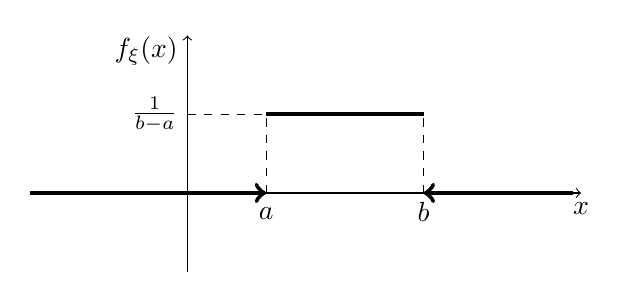
\begin{tikzpicture}[yscale = 2]
        \pgfmathsetmacro{\a}{1};
        \pgfmathsetmacro{\b}{3};
        \draw [->] (-2, 0) -- (5, 0);
        \draw [->] (0, -0.5) -- (0, 1);
        \draw [ultra thick] (\a, {1/(\b -\a)}) -- (\b, {1/(\b -\a)});
        \draw [dashed] (\a, 0) -- (\a, {1/(\b -\a)});
        \draw [dashed] (\b, 0) -- (\b, {1/(\b -\a)});
        \draw [ultra thick] [->] (-2, 0) -- (\a, 0);
        \draw [ultra thick] [<-] (\b, 0) -- (4.9, 0);
        \node [below] at (\a, -0.03) {$a$};
        \node [below] at (\b, 0) {$b$};
        \draw [dashed] (0, {1/(\b -\a)}) -- (\a, {1/(\b -\a)});
        \node [left] at (0, {1/(\b -\a)}) {$\frac{1}{b-a}$};
        \node [below] at (5, 0) {$x$};
        \node [left] at (0, 0.9) {$f_\xi(x)$};
    \end{tikzpicture}
\end{center}

\noindent \textbf{Функція розподілу:}
\begin{center}
    \begin{tabular}{c c}
        $
            F_\xi(x) = \begin{cases}
                0, & x \leq a \\
                \frac{x-a}{b-a}, & a< x \leq b \\
                1, & x > b
            \end{cases}
        $ &
        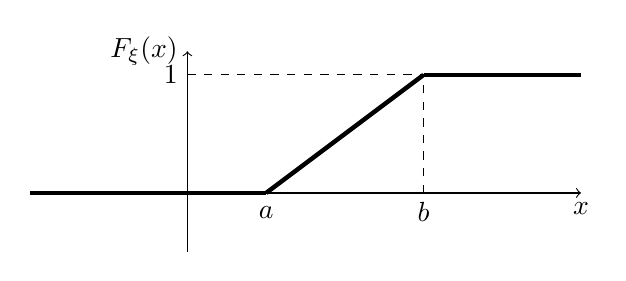
\begin{tikzpicture}[baseline={(current bounding box.center)}, yscale=1.5]
            \pgfmathsetmacro{\a}{1};
        \pgfmathsetmacro{\b}{3};
        \draw [->] (-2, 0) -- (5, 0);
        \draw [->] (0, -0.5) -- (0, 1.2);
        \draw [ultra thick] (-2, 0) -- (\a, 0);
        \draw [domain=\a:\b, smooth, variable = \x, ultra thick] plot ({\x}, {(\x-\a)/(\b-\a)});
        \draw [ultra thick] (\b, 1) -- (5, 1);
        \node [below] at (\a, -0.03) {$a$};
        \node [below] at (\b, 0) {$b$};
        \node [below] at (5, 0) {$x$};
        \node [left] at (0, 1.2) {$F_\xi(x)$};
        \draw [dashed] (0, 1) -- (\b, 1);
        \draw [dashed] (\b, 0) -- (\b, 1);
        \node [left] at (0, 1) {$1$};
        %\node [right] [align=center] at (2.5, 0.3) {Приклад для \\ $a = \a, b = \b$};
        \end{tikzpicture}
    \end{tabular}
\end{center}

\noindent\textbf{Числові характеристики:}
\begin{enumerate}
    \item $\E\xi = \int\limits_{-\infty}^{+\infty} x f_\xi(x)dx = \int\limits_{a}^{b} \frac{x}{b-a}dx = \frac{a+b}{2}$.
    \item $\D\xi = \E\xi^2 - (\E\xi)^2 = \int\limits_{a}^{b} \frac{x^2}{b-a}dx - \frac{(a+b)^2}{4} = \frac{(b-a)^2}{12}$, $\sigma_\xi = \frac{b-a}{2\sqrt{3}}$.
    \item ${Mo}\xi$ --- будь-яка точка з $\left<a; b\right>$.
    \item ${Me}\xi = \frac{a+b}{2}$.
    \item ${As}\xi = 0$.
    \item ${Ex}\xi = -\frac{6}{5}$.
\end{enumerate}

\noindent\textbf{Застосування:} отримання вибірок з інших законів розподілу;
похибка округлення до найближчої поділки приладу при ціні поділки $a$ має розподіл $\mathrm{U}\left<-\frac{a}{2}; \frac{a}{2}\right>$.

\subsection{Експоненційний (показниковий) розподіл}
\noindent\textbf{Означення:}
    НВВ $\xi$ розподілена за \emph{експоненційним законом}, 
    якщо її щільність розподілу має вигляд \begin{equation}
        f_\xi(x) = \begin{cases}
            \lambda e^{-\lambda x}, & x \geq 0 \\
            0, & x < 0
        \end{cases}
    \end{equation}
\textbf{Коротке позначення:} $\xi \sim \mathrm{Exp}(\lambda)$.
    $\lambda > 0$ --- параметр закону.

\noindent \textbf{Крива розподілу:}
\begin{center}
    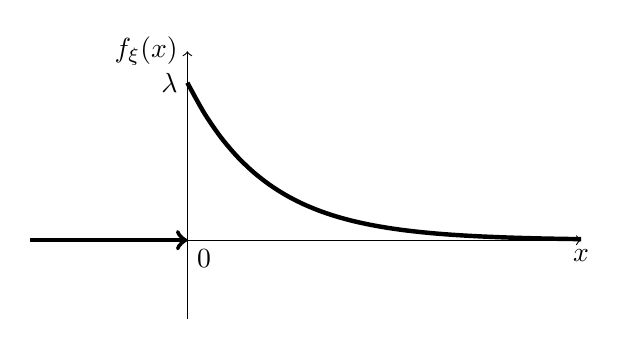
\begin{tikzpicture}[yscale = 2]
        \pgfmathsetmacro{\l}{1};
        \draw [->] (-2, 0) -- (5, 0);
        \draw [->] (0, -0.5) -- (0, 1.2);
        \draw [ultra thick] [->] (-2, 0) -- (0, 0);
        \draw [domain=0:5, smooth, variable = \x, ultra thick] plot ({\x}, {\l*e^(-\l*\x)});
        \node [below] at (5, 0) {$x$};
        \node [left] at (0, 1.2) {$f_\xi(x)$};
        \node [below right] at (0, 0) {$0$};
        \node [left] at (0, \l) {$\lambda$};
    \end{tikzpicture}
\end{center}

\noindent \textbf{Функція розподілу:}
\begin{center}
    \begin{tabular}{c c}
        $
            F_\xi(x) = \begin{cases}
                \lambda \int\limits_0^x e^{-\lambda t} dt = 1 - e^{-\lambda x}, & x> 0 \\
                0, & x \leq 0
            \end{cases}
            $ &
        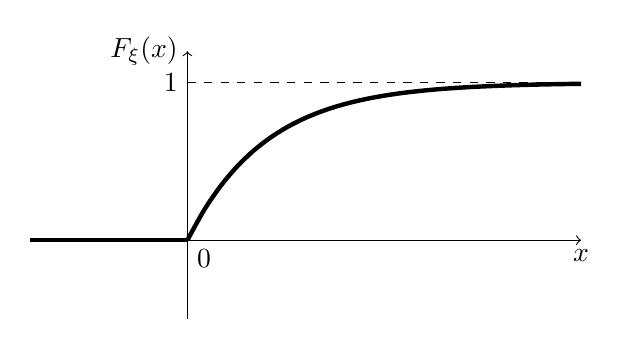
\begin{tikzpicture}[baseline={(current bounding box.center)}, yscale=2]
            \pgfmathsetmacro{\l}{1};
            \draw [->] (-2, 0) -- (5, 0);
            \draw [->] (0, -0.5) -- (0, 1.2);
            \draw [ultra thick] (-2, 0) -- (0, 0);
            \draw [domain=0:5, smooth, variable = \x, ultra thick] plot ({\x}, {1 - e^(-\l*\x)});
            \node [below] at (5, 0) {$x$};
            \node [left] at (0, 1.2) {$F_\xi(x)$};
            \node [below right] at (0, 0) {$0$};
            \node [left] at (0, 1) {$1$};
            \draw [dashed] (0, 1) -- (5, 1);
        \end{tikzpicture}
    \end{tabular}
\end{center}

Знайдемо всі \emph{початкові моменти} експоненційного розподілу.

$\E\xi^k = \int\limits_{-\infty}^{+\infty} x^k f_\xi(x)dx = \lambda \int\limits_{0}^{+\infty} x^k e^{-\lambda x}dx = \left[ \lambda x = t, dx = \frac{dt}{\lambda}\right]=
\frac{\lambda}{\lambda^k \cdot \lambda} \int\limits_{0}^{+\infty} t^k e^{-t} dt = \frac{\Gamma(k+1)}{\lambda^k} = \frac{k!}{\lambda^k}$.

\noindent\textbf{Числові характеристики:}
\begin{enumerate}
    \item $\E\xi = \frac{1}{\lambda}$.
    \item $\D\xi = \E\xi^2 - (\E\xi)^2 = \frac{2}{\lambda^2} - \frac{1}{\lambda^2} = \frac{1}{\lambda^2}$, $\sigma_\xi = \frac{1}{\lambda}$.
    \item ${Mo}\xi = 0$.
    \item ${Me}\xi = \frac{\ln2}{\lambda}$.
    \item ${As}\xi = 2$ --- не залежить від $\lambda$, бо $\beta_3 = \alpha_3 - 3\alpha_2 \alpha_1 + 2 \alpha_1^3 = \frac{2}{\lambda^3}$.
    \item ${Ex}\xi = 6$.
\end{enumerate}

\begin{exercise}
    Дослідити характеристики інших варіантів експоненційного розподілу:
    $\mathrm{Exp}(\lambda, x_0)$ з щільністю $f_\xi(x) = \begin{cases}
        \lambda e^{-\lambda (x-x_0)}, & x \geq x_0 \\
        0, & x < x_0
    \end{cases}$ (експоненційний із зсувом) та $\mathrm{Exp}(\alpha)$ зі щільністю
    $f_\xi(x) = \begin{cases}
        \frac{1}{\alpha} e^{-\frac{x}{\alpha}}, & x \geq 0 \\
        0, & x < 0
    \end{cases}$, що відповідає розглянутому варіанту, але з параметром $\lambda = \frac{1}{\alpha}$.
\end{exercise}

Як і геометричний розподіл, експоненційний \textbf{<<не має пам'яті>>}.
Доведемо: якщо проміжок часу $T$, розподілений за експоненційним законом,
тягнувся час $\tau$, то проміжок $T_1 = T - \tau$ розподілений так само --- 
за експоненційним законом з тим самим параметром.
\begin{gather*}
    F_{T_1}(t) = \P\left\{T_1 < t / T \geq \tau\right\} = 
    \frac{\P\left\{(T_1 < t) \cap (T \geq \tau)\right\}}{\P\left\{ T \geq \tau \right\}} =
    \frac{\P{\left\{\tau \leq T < t +\tau\right\}}}{1 - \P\left\{ T < \tau \right\}} = \\
    \frac{F_T(t+\tau) - F_T(\tau)}{1-F_T(\tau)} = 
    \frac{1-e^{-\lambda (t+\tau)} - (1 - e^{-\lambda \tau})}{1-(1-e^{-\lambda \tau})} =
    \frac{e^{-\lambda \tau}(1-e^{-\lambda t})}{e^{-\lambda \tau}} = 1-e^{-\lambda t}
\end{gather*}
Отже, $F_{T_1}(t) = F_T(t)$.

\noindent\textbf{Застосування:}
\begin{enumerate}
    \item Час між двома сусідніми подіями в потоці Пуассона має експоненційний розподіл.
    \begin{exercise}
        Довести цю властивість.
    \end{exercise}
    \item Як правило, час безвідмовної роботи приладу має експоненційний розподіл.
    
    Нехай в момент часу $t=0$ увімкнули прилад. Припустимо, що умовна ймовірність виходу з ладу
    приладу в інтервалі часу $\left[ t; t+\Delta t\right)$ за умови, що до часу $t$ він працював,
    пропорційна $\Delta t$ і рівна $\lambda\cdot \Delta t + o(\Delta t)$. Нехай $\xi$ --- час безвідмовної роботи,
    покладемо $Q(t) = \P\left\{\xi \geq t\right\}$.
    $Q(t+\Delta t) = \P\left\{\xi \geq t + \Delta t\right\} = \P\left\{\xi \geq t\right\} \cdot \P\left\{\xi \geq t+\Delta t / \xi \geq t\right\} = 
    Q(t) \cdot (1 - \lambda\cdot \Delta t + o(\Delta t))$.
    $\frac{Q(t+\Delta t) - Q(t)}{\Delta t} = -\lambda Q(t) + \frac{o(\Delta t)}{\Delta t} \cdot Q(t)$,
    при $\Delta t \rightarrow 0$ отримаємо $Q'(t) = -\lambda Q(t)$.
    Розв'язком цього диференціального рівняння буде $Q(t) = C\cdot e^{-\lambda t}$.
    Оскільки вважаємо, що в момент часу $t=0$ прилад працював, то $Q(0) = 1$ і $C=1$.

    Тоді $F_\xi(t) = \P\left\{ \xi < t\right\} = 1 - \P\left\{ \xi \geq t\right\} = 1 - Q(t) = \begin{cases}
        1 - e^{-\lambda t}, & t \geq 0 \\
        0, & t < 0
    \end{cases}$. Отже, $\xi \sim \mathrm{Exp}(\lambda)$.
\end{enumerate}

\begin{example}
    Яка ймовірність того, що людина проживе 100 років? Нехай $\xi$ --- час життя людини.
    Оскільки $\P\left\{\xi = 100\right\} = 0$, знайдемо $\P\left\{ \xi \geq 100\right\}$.
    $\P\left\{ \xi \geq 100\right\} = e^{-\lambda \cdot 100}$, $\lambda = \text{?}$.
    Оскільки $\lambda = \frac{1}{\E\xi}$, то, прийнявши $\E\xi = 70$ (середня тривалість життя),
    отримаємо $\P\left\{ \xi \geq 100\right\} = e^{-100/70} \approx 0.24$.
\end{example}

\subsection{Гауссівський (нормальний) розподіл}
\noindent\textbf{Означення:}
    НВВ $\xi$ розподілена за \emph{нормальним законом}, 
    якщо її щільність розподілу має вигляд 
    \begin{equation}
        f_\xi(x) = \frac{1}{\sqrt{2\pi}\sigma} e^{-\frac{(x-a)^2}{2\sigma^2}}
    \end{equation}
\textbf{Коротке позначення:} $\xi \sim \mathrm{N}(a, \sigma)$ або 
    $\xi \sim \mathrm{N}(a, \sigma^2)$.
    $a \in \mathbb{R}, \sigma > 0$ --- параметри закону.

    Розподіл $\mathrm{N}(0, 1)$ називають стандартним гауссівським розподілом.

\noindent \textbf{Крива розподілу:}
\begin{center}
    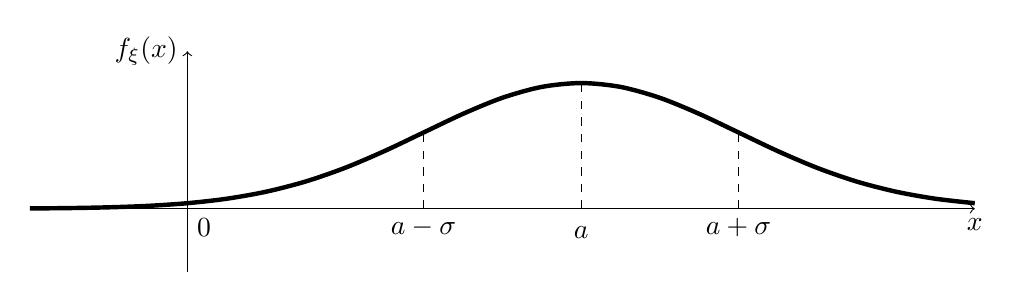
\begin{tikzpicture}[yscale = 4, xscale = 2]
        \pgfmathsetmacro{\a}{2.5};
        \pgfmathsetmacro{\s}{1}
        \draw [->] (-1, 0) -- (5, 0);
        \draw [->] (0, -0.2) -- (0, 0.5);
        \draw [dashed] (\a, 0) -- (\a, 0.398942280401/\s);
        \draw [dashed] (\a-\s, 0) -- (\a-\s, 0.241970724519/\s);
        \draw [dashed] (\a+\s, 0) -- (\a+\s, 0.241970724519/\s);
        \draw [domain=-1:5, smooth, variable = \x, ultra thick] plot ({\x}, {0.398942280401/\s * e^(-(\x-\a)^2/(2*\s^2))});
        \node [below] at (5, 0) {$x$};
        \node [below] at (\a, -0.025) {$a$};
        \node [below] at (\a-\s, 0) {$a - \sigma$};
        \node [below] at (\a+\s, 0) {$a + \sigma$};
        \node [below right] at (0, 0) {$0$};
        \node [left] at (0, 0.5) {$f_\xi(x)$};
    \end{tikzpicture}
\end{center}

\noindent \textbf{Зміст параметрів $a$ та $\sigma^2$:}
\begin{enumerate}
    \item $\E\xi = 
    \frac{1}{\sqrt{2\pi}\sigma}
    \int\limits_{-\infty}^{+\infty}x e^{-\frac{(x-a)^2}{2\sigma^2}} dx 
    = \left[ \frac{x-a}{\sigma \sqrt{2}} = t, \; dx = \sigma\sqrt{2}dt \right] = 
    \frac{1}{\sqrt{\pi}}\int\limits_{-\infty}^{+\infty} 
    (a + \sigma\sqrt{2}t)e^{-t^2} dt =$
    
    $=\frac{a}{\sqrt{\pi}}
    \int\limits_{-\infty}^{+\infty}e^{-t^2}dt =
    \left[\text{інтеграл Ейлера-Пуассона}\right] = a$.
    \item Знайдемо всі центральні моменти:
    $\beta_k = \E(\xi - \E\xi)^k = 
    \frac{1}{\sigma\sqrt{2\pi}}
    \int\limits_{-\infty}^{+\infty}(x-a)^k 
    e^{-\frac{(x-a)^2}{2\sigma^2}} dx = \left[
        \text{ідентична заміна}
    \right] =
    \frac{\sigma^k 2^{k/2}}{\sqrt{\pi}}
    \int\limits_{-\infty}^{+\infty}t^k 
    e^{-t^2} dt
    $.

    Якщо $k = 2l + 1$, то $\beta_k = 0$ (непарна функція під інтегралом).
    $\beta_3 = 0 \Rightarrow As\xi = 0$.

    Візьмемо $k = 2l$:

    $\beta_{2l} = 
    \frac{\sigma^{2l} 2^{l}}{\sqrt{\pi}}
    \int\limits_{-\infty}^{+\infty}t^{2l} 
    e^{-t^2} dt = 
    \left[ t^2 = z, \; dt = \frac{1}{2} z^{-\frac{1}{2}}dz\right] =
    2\frac{\sigma^{2l}2^l}{\sqrt{\pi}}
    \int\limits_{0}^{+\infty}z^l e^{-z}\cdot \frac{1}{2} z^{-\frac{1}{2}}
    dz = $
    
    $= \frac{\sigma^{2l}2^l}{\sqrt{\pi}}
    \int\limits_{0}^{+\infty}z^{l-\frac{1}{2}} e^{-z}
    dz = 
    \frac{\sigma^{2l}2^l}{\sqrt{\pi}}\cdot\Gamma(l+\frac{1}{2})$.
\end{enumerate}

\noindent \textbf{Числові характеристики:}
\begin{enumerate}
    \item $\E\xi = Mo\xi = Me\xi = a$.
    \item $\D\xi = \frac{2 \sigma^2}{\sqrt{\pi}}\cdot\Gamma\left(\frac{3}{2}\right) 
    = \sigma^2$, $\sigma_\xi = \sigma$.
    \item $As\xi = 0$.
    \item $Ex\xi = \frac{\beta_4}{\sigma_\xi^4} - 3 = 
    \frac{\sigma^4\cdot2^2\cdot\Gamma(5/2)}{\sqrt{\pi}\cdot\sigma^4} - 3 = \frac{4\cdot\sqrt{\pi}\cdot 3/4}{\sqrt{\pi}} - 3 = 0$. 
    Доданок $-3$ у формулі ексцесу був введений саме для того, щоб нормальний розподіл мав нульовий ексцес.
\end{enumerate}

\noindent \textbf{Функція розподілу:}

$F_\xi(x) = \int\limits_{-\infty}^{x} f_\xi(t) dt = 
\frac{1}{\sqrt{2\pi}\sigma} \int\limits_{-\infty}^{x} 
e^{-\frac{(t-a)^2}{2\sigma^2}} dt$ --- не береться в елементарних 
функціях.

Для зручного використання гауссівського закону в задачах введемо 
спеціальну функцію, значення якої занесено до таблиць.

\noindent \textbf{Функція Лапласа:}


\begin{tabular}{c c}
    $
        \Phi(x) = \frac{1}{\sqrt{2\pi}} 
        \int\limits_{0}^{x} e^{-\frac{t^2}{2}} dt
    $
    &
    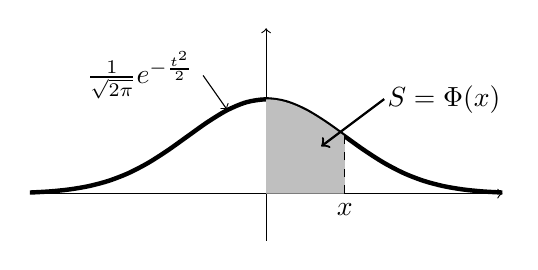
\begin{tikzpicture}[baseline={(current bounding box.center)}, yscale=3, 
        scale = 1]
        \draw [->] (-3, 0) -- (3, 0);
        \draw [->] (0, -0.2) -- (0, 0.7);
        \draw [domain=-3:3, smooth, variable = \x, ultra thick] plot ({\x}, 
        {
            (0.3989422804) * e^(- (\x * \x / 2))
        });
        \fill [lightgray, domain=0:1, smooth, variable = \x] plot ({\x}, 
        {
            (0.3989422804) * e^(- (\x * \x / 2))
        }) -- (1, 0) -- (0, 0) -- (0, 0.3989422804);
        \node [below] at (1, 0) {$x$};
        \draw [dashed] (1, 0) -- (1, 0.25);
        \draw [->, thick] (1.5, 0.4) -- (0.7, 0.2);
        \node [below left] at (3.1, 0.5) {$S = \Phi(x)$};
        \draw [->] (-0.8, 0.5) -- (-0.495, 0.355);
        \node [left] at (-0.8, 0.5) {$\frac{1}{\sqrt{2\pi}}e^{-\frac{t^2}{2}}$};
    \end{tikzpicture}
\end{tabular}

\noindent
\begin{tabular}{p{0.5\textwidth} c}
    \emph{Властивості функції Лапласа: }
    \begin{enumerate}
        \item $\Phi(-x) = -\Phi(x)$ --- непарна.
        \item $\Phi(0) = 0$.
        \item $y = \pm 0.5$ --- горизонтальні асимптоти.
        \item $\forall x \geq 5: \Phi(x) \approx 0.5 $.
        \item $\forall x \leq -5: \Phi(x) \approx -0.5 $.
    \end{enumerate}
    &
    \adjustbox{valign=t}
    {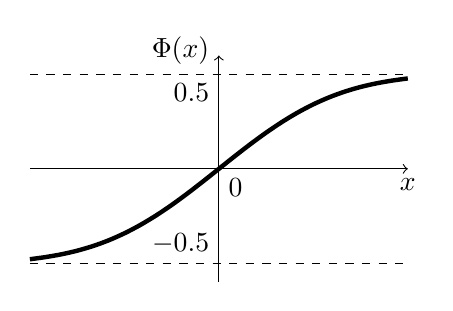
\begin{tikzpicture}[yscale=2, scale = 1.2]
        \draw [->] (-2, 0) -- (2, 0);
        \draw [->] (0, -0.6) -- (0, 0.6);
        \draw [domain=-2:2, smooth, variable = \x, ultra thick] plot ({\x}, 
        {
            (0.564189583547756) * (
            (\x / 1.414213562373095) 
            - ((\x / 1.414213562373095)^3 / 3) 
            + ((\x / 1.414213562373095)^5 / 10) 
            - ((\x / 1.414213562373095)^7 / 42)
            + ((\x / 1.414213562373095)^9 / 216) 
            - ((\x / 1.414213562373095)^11 / 1320)
            + ((\x / 1.414213562373095)^13 / 9360)
            )
        });
        \node [below] at (2, 0) {$x$};
        \node [above left] at (0, 0.5) {$\Phi(x)$};
        \node [below right] at (0, 0) {$0$};
        \draw [dashed] (-2, -0.5) -- (2, -0.5);
        \draw [dashed] (-2, 0.5) -- (2, 0.5);
        \node [below left] at (0, 0.5) {$0.5$};
        \node [above left] at (0, -0.5) {$-0.5$};
    \end{tikzpicture}}
\end{tabular}

\noindent Виразимо функцію розподілу гауссівського закону через функцію Лапласа:
\begin{equation}
    F_\xi (x) = \frac{1}{\sqrt{2\pi}\sigma} \int\limits_{-\infty}^{x} 
    e^{-\frac{(t-a)^2}{2\sigma^2}} dt = 
    \left[\frac{t-a}{\sigma} = z\right] = 
    \frac{1}{\sqrt{2\pi}} \int\limits_{-\infty}^{\frac{x-a}{\sigma}} 
    e^{-\frac{z^2}{2}} dz = \frac{1}{2} + 
    \Phi\left(\frac{x-a}{\sigma}\right)
\end{equation}

\noindent \textbf{Робочі формули для розв'язання задач:}
\begin{enumerate}
    \item $\P\left\{\xi \in \left<\alpha; \beta\right>\right\} 
    = F_\xi(\beta) - F_\xi(\alpha) = \Phi\left(\frac{\beta - a}{\sigma}\right)
    - \Phi\left(\frac{\alpha - a}{\sigma}\right)$.
    \item $\P\left\{\left| \xi - a \right| < \varepsilon\right\} = 
    \P\left\{\xi \in \left(a - \varepsilon, a + \varepsilon\right)\right\} = 
    \Phi\left(\frac{a + \epsilon - a}{\sigma}\right)
    - \Phi\left(\frac{a - \epsilon - a}{\sigma}\right) = 
    2\Phi(\frac{\varepsilon}{\sigma})$.
    \item \emph{<<Правило $3\sigma$>>}: 
    $\P\left\{\left| \xi - a \right| < 3\sigma\right\} = 
    \P\left\{\xi \in \left( a-3\sigma; a+3\sigma\right)\right\} = 2\Phi\left(3\right)
    \approx 0.9973$.

    Майже всі значення випадкової величини, розподіленої за 
    гауссівським законом, лежать на відстані не більше трьох середньоквадратичних 
    відхилень від її математичного сподівання.
\end{enumerate}

\subsection{Гамма-розподіл}
\noindent\textbf{Означення:}
    НВВ $\xi$ розподілена за \emph{гамма-законом}, 
    якщо її щільність розподілу має вигляд 
    \begin{equation}
        f_\xi(x) = \begin{cases}
            \frac{\beta^\alpha}{\Gamma(\alpha)} x^{\alpha-1} e^{-\beta x}, & x \geq 0 \\
            0, & x < 0
        \end{cases}
    \end{equation}
\textbf{Коротке позначення:} $\xi \sim {\Gamma}(\alpha, \beta)$.
    $\alpha >0, \beta > 0$ --- параметри закону.
\begin{remark}
    ${\Gamma}(1, \lambda) = \mathrm{Exp}(\lambda)$.
\end{remark}
\noindent \textbf{Крива розподілу:}

\begin{center}
    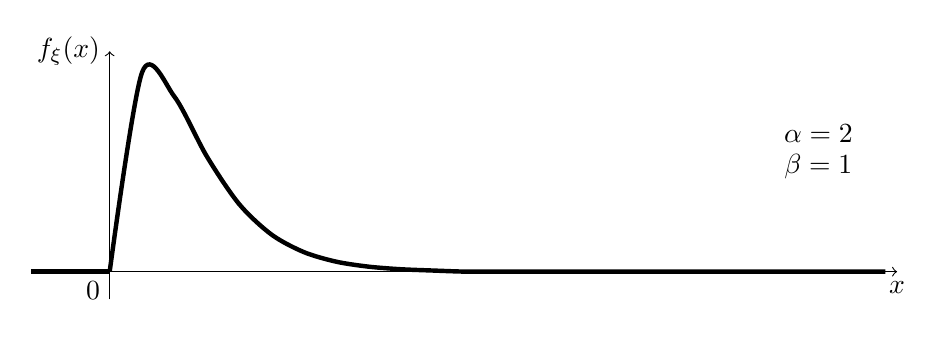
\begin{tikzpicture}[yscale = 7, xscale = 0.5, baseline={(current bounding box.center)}]
        \pgfmathsetmacro{\a}{2};
        \pgfmathsetmacro{\b}{1};
        \draw [->] (-2, 0) -- (20, 0);
        \draw [->] (0, -0.05) -- (0, 0.4);
        \draw [ultra thick] (-2, 0) -- (0, 0);
        \draw [domain=0:19.7, smooth, variable = \x, ultra thick] plot ({\x}, {\b^(\a)*\x^(\a-1) * e^(-\x*\b)});
        \node [below] at (20, 0) {$x$};
        \node [left] at (0, 0.4) {$f_\xi(x)$};
        \node [below left] at (0, 0) {$0$};
        \node at (18, 0.25) {$\alpha = 2$};
        \node at (18, 0.19) {$\beta = 1$};
    \end{tikzpicture} 
\end{center}

\begin{center}
    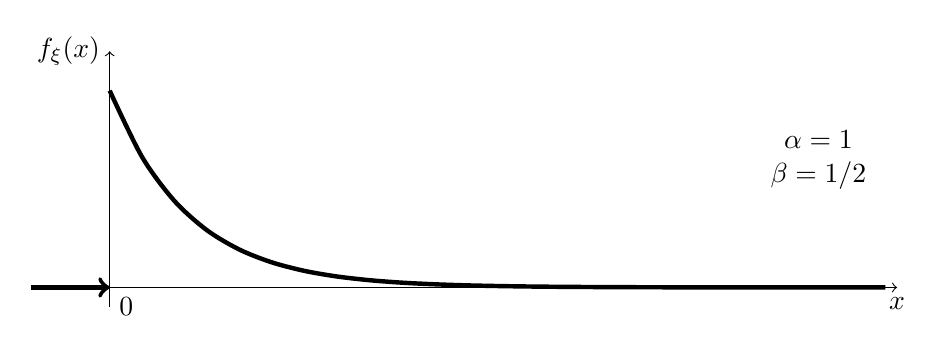
\begin{tikzpicture}[yscale = 5, xscale = 0.5, baseline={(current bounding box.center)}]
        \pgfmathsetmacro{\a}{1};
        \pgfmathsetmacro{\b}{0.5};
        \draw [->] (-2, 0) -- (20, 0);
        \draw [->] (0, -0.05) -- (0, 0.6);
        \draw [ultra thick] [->] (-2, 0) -- (0, 0);
        \draw [domain=0:19.7, smooth, variable = \x, ultra thick] plot ({\x}, {\b^(\a)*\x^(\a-1) * e^(-\x*\b)});
        \node [below] at (20, 0) {$x$};
        \node [left] at (0, 0.6) {$f_\xi(x)$};
        \node [below right] at (0, 0) {$0$};
        \node at (18, 0.375) {$\alpha = 1$};
        \node at (18, 0.285) {$\beta = 1/2$};
    \end{tikzpicture} 
\end{center}

\noindent \textbf{Функція розподілу:}
\nopagebreak

\begin{tabular}{c c}
    \begin{tabular}{c}
        $
        F_\xi(x) = \begin{cases}
            0, & x \leq 0 \\
            \int\limits_0^x f_\xi(t)dt = \frac{\gamma(\alpha, \beta x)}{\Gamma(\alpha)}, & x>0 
        \end{cases}$
        \\
        де $\gamma(s, x) = \int\limits_0^x t^{s-1} e^{-t} dt$
    \end{tabular}
    &
    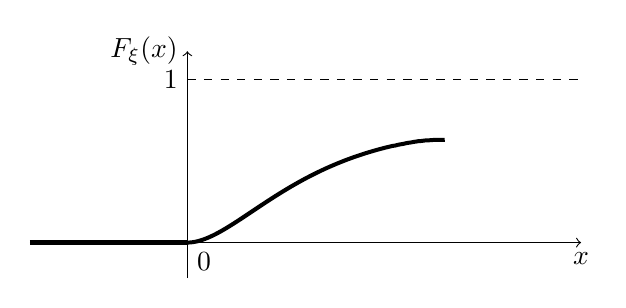
\begin{tikzpicture}[baseline={(current bounding box.center)}, yscale=0.9]
        \pgfmathsetmacro{\a}{2};
        \pgfmathsetmacro{\b}{3};
        \draw [->] (-2, 0) -- (5, 0);
        \draw [->] (0, -0.5) -- (0, 2.7);
        \draw [ultra thick] (-2, 0) -- (0, 0);
        \draw [dashed] (0, 2.3) -- (5, 2.3);
        \node [below] at (5, 0) {$x$};
        \node [left] at (0, 2.7) {$F_\xi(x)$};
        \node [left] at (0, 2.3) {$1$};
        \node [below right] at (0, 0) {$0$};
        \begin{axis}[width=0.4\textwidth,height=0.25\textwidth, samples=100, domain = 0:4, restrict y to domain = 0:1, axis x line=bottom,axis y line=left, clip=false, axis line style={draw=none}, ticks=none]
        \addplot [ultra thick] plot ({\x}, {(\x^\a) * (
            1/\a -
            \x/(1+\a) +
            \x^2/(2*(2+\a)) -
            \x^3/(6*(3+\a)) +
            \x^4/(24*(4+\a)) -
            \x^5/(120*(5+\a)) +
            \x^6/(720*(6+\a)) -
            \x^7/(5040*(7+\a)) +
            \x^8/(40320*(8+\a)) -
            \x^9/(362880*(9+\a)) +
            \x^10/(3628800*(10+\a)) -
            \x^11/(39916800*(11+\a))
        )});
        \end{axis}
    \end{tikzpicture}
\end{tabular}

Знайдемо всі \emph{початкові моменти} гамма-розподілу.

$\E\xi^k = \int\limits_{-\infty}^{+\infty} x^k f_\xi(x)dx = \frac{\beta^\alpha}{\Gamma(\alpha)} \int\limits_0^{+\infty} x^k x^{\alpha-1} e^{-\beta x} dx = 
\left[ \beta x = t\right] = \frac{\beta^\alpha}{\Gamma(\alpha)} \cdot \frac{1}{\beta^k\cdot \beta^{\alpha}} \int\limits_0^{+\infty} t^{k+\alpha-1} e^{-t} dt = 
\frac{1}{\Gamma(\alpha) \cdot \beta^k} \int\limits_0^{+\infty} t^{k+\alpha-1} e^{-t} dt = \frac{\Gamma(\alpha+k)}{\Gamma(\alpha) \cdot \beta^k}$.
Зокрема, $\E\xi = \frac{\Gamma(\alpha+1)}{\Gamma(\alpha) \cdot \beta} = \frac{\alpha}{\beta}$,
$\E\xi^2 = \frac{\Gamma(\alpha+2)}{\Gamma(\alpha) \cdot \beta^2}  = \frac{(\alpha+1)\alpha}{\beta^2}$.

\noindent\textbf{Числові характеристики:}
\begin{enumerate}
    \item $\E\xi = \frac{\alpha}{\beta}$.
    \item $\D\xi = \E\xi^2 - (\E\xi)^2 = \frac{(\alpha+1)\alpha}{\beta^2} - \frac{\alpha^2}{\beta^2} = \frac{\alpha}{\beta^2}$, $\sigma_\xi = \frac{\sqrt{\alpha}}{\beta}$.
    \item ${Mo}\xi = \frac{\alpha-1}{\beta}$.
    \item ${Me}\xi$ --- немає виразу у замкненій формі.
    \item ${As}\xi = \frac{2}{\sqrt{\alpha}}$.
    \item ${Ex}\xi = \frac{6}{\alpha}$.
\end{enumerate}

\noindent\textbf{Застосування:} гамма-розподіл застосовується для моделювання
складних потоків подій, в економіці, теорії масового обслуговування, логістиці.
У випадку натурального параметру $\alpha = k \in \mathbb{N}$ за законом
$\Gamma(k, \lambda)$ розподілений час очікування появи $k$-тої події
в процесі Пуассона з інтенсивністю $\lambda$. Така версія гамма-розподілу називається \emph{розподілом Ерланга}.
\begin{exercise}
    Нехай $T$ --- час очікування появи $k$-тої події
    в процесі Пуассона з інтенсивністю $\lambda$. Довести $T \sim \Gamma(k, \lambda)$.
\end{exercise} % https://towardsdatascience.com/gamma-distribution-intuition-derivation-and-examples-55f407423840